
%2.1
\section{Automatic Identification of Software Bugs}
Classification of bug detection tools.\\
The following table needs to be customized\\
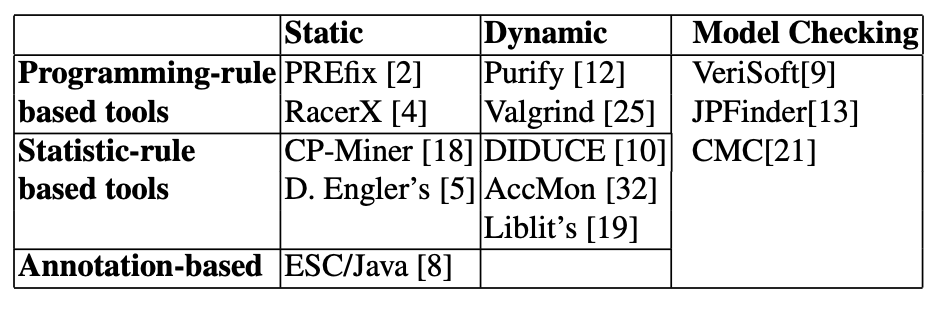
\includegraphics{classification-of-bug-detection-tools.png}
\\
\textbf{PREfix} is a source code analyzer that detects a broad range of errors in C and C++ code \cite{bush2000static}.
Its goal is to detect many runtime issues on real world programs, without dynamic analysis and instrumentation; only the source code text is used. PREfix can detect defects efficiently through a model that abstracts functions and their interactions; the analyzer traces execution paths handling multiple language features: pointers, arrays, structs, bit field operations, control flows statements and so on.
The method used is based on the simulation of individual functions; it uses a virtual machine that simulates the actions of each operator and function call. With the detailed tracking it can report defects information to the user so to easily characterize the detected error.
The tool can be applied both to a complete program source or only a subset. This bottom up approach is particularly useful when the source code is not fully available (e.g. in the case of a thirty part library).
\\
\\
\textbf{RacerX} deals with complex multithread systems. It detects race conditions and deadlock using static analysis \cite{engler2003racerx}.
The tool can infer from the source code the object lock that is assigned to a particular code block. It detects code that is multithreaded and the code that apply dangerous shared access. 
RaceX uses annotations only to mark the code that deals with lock acquisition; this requirement keeps the burden on the user to the minimum to increase ease of adoption. The authors of RaceX report their experiences on the biggest problem about race detection: in large codebase there are massive amounts of unprotected variable access; the key point is to report only those that can actually cause problems. There is emphasis on two aspects. The first is to minimize the impact of reporting false positive in order to avoid the users to discard the use of the tool; to achieve this, RaceX employs specific techniques to lower the impact of analysis mistakes. The second is the speed of the tool: the authors keep the time of execution for the analysis under deep scrutiny; they claim that for a codebase of 1.8 LOC the time required is between 2-14 minutes. The tool has been found capable of finding sever problems in huge projects like Linux, FreeBSD and a large closed source commercial software.
\\
\\

\textbf{Purify}
 is a dynamic  analysis tool for software testing and quality assurance \cite{hastings1992fast}. 
 It instruments the object code files generated from compilers (the software dates back to 1992 and the supported platform is Sun Microsystem's SPARC); the target object files include also third-party libraries. Purify detects multiple errors: memory leaks, access error, reading uninitialized memory. The injected instructions check every read and write memory operations; the slow down of the target is under three times in respect to the non-instrumented execution time. The authors emphasizes: the ease of use in the classic makefile development toolchain and the low overhead that allows the developer to detect bugs early on in the development cycle.
\\
\\
\textbf{Valgrind [25] todo: this is copy\&paste of the website description and wikipedia}
Valgrind is an instrumentation framework for building dynamic analysis tools. There are Valgrind tools that can automatically detect many memory management and threading bugs, and profile your programs in detail. You can also use Valgrind to build new tools.

[wikipedia]
Valgrind is in essence a virtual machine using just-in-time (JIT) compilation techniques, including dynamic recompilation. Nothing from the original program ever gets run directly on the host processor. Instead, Valgrind first translates the program into a temporary, simpler form called Intermediate Representation (IR), which is a processor-neutral, SSA-based form. After the conversion, a tool (see below) is free to do whatever transformations it would like on the IR, before Valgrind translates the IR back into machine code and lets the host processor run it. Valgrind recompiles binary code to run on host and target (or simulated) CPUs of the same architecture. It also includes a GDB stub to allow debugging of the target program as it runs in Valgrind, with "monitor commands" that allow you to query the Valgrind tool for various sorts of information.

A considerable amount of performance is lost in these transformations (and usually, the code the tool inserts); usually, code run with Valgrind and the "none" tool (which does nothing to the IR) runs at 1/4 to 1/5 of the speed of the normal program.
\\
\\
\textbf{CP-Miner [18] todo: this is copy\&paste of the paper abstract}
Copy-pasted code is very common in large software be- cause programmers prefer reusing code via copy-paste in order to reduce programming effort. Recent studies show that copy-paste is prone to introducing bugs and a sig- nificant portion of operating system bugs concentrate in copy-pasted code. Unfortunately, it is challenging to ef- ficiently identify copy-pasted code in large software. Ex- isting copy-paste detection tools are either not scalable to large software, or cannot handle small modifications in copy-pasted code. Furthermore, few tools are available to detect copy-paste related bugs.
In this paper we propose a tool, CP-Miner, that uses data mining techniques to efficiently identify copy-pasted code in large software including operating systems, and detects copy-paste related bugs. Specifically, it takes less than 20 minutes for CP-Miner to identify 190,000 copy- pasted segments in Linux and 150,000 in FreeBSD. More- over, CP-Miner has detected 28 copy-paste related bugs in the latest version of Linux and 23 in FreeBSD. In addition, we analyze some interesting characteristics of copy-paste in Linux and FreeBSD, including the distribution of copy- pasted code across different length, granularity, modules, degrees of modification, and various software versions.
\\
\\
\textbf{D. Engler's [5] todo: this is copy\&paste of the paper abstract}
A major obstacle to finding program errors in a real system is knowing what correctness rules the system must obey. These rules are often undocumented or specified in an ad hoc manner. This paper demonstrates techniques that automatically extract such checking information from the source code itself, rather than the programmer, thereby avoiding the need for a priori knowledge of system rules.The cornerstone of our approach is inferring programmer "beliefs" that we then cross-check for contradictions. Beliefs are facts implied by code: a dereference of a pointer, p, implies a belief that p is non-null, a call to "unlock(1)" implies that 1 was locked, etc. For beliefs we know the programmer must hold, such as the pointer dereference above, we immediately flag contradictions as errors. For beliefs that the programmer may hold, we can assume these beliefs hold and use a statistical analysis to rank the resulting errors from most to least likely. For example, a call to "spin\_lock" followed once by a call to "spin\_unlock" implies that the programmer may have paired these calls by coincidence. If the pairing happens 999 out of 1000 times, though, then it is probably a valid belief and the sole deviation a probable error. The key feature of this approach is that it requires no a priori knowledge of truth: if two beliefs contradict, we know that one is an error without knowing what the correct belief is.Conceptually, our checkers extract beliefs by tailoring rule "templates" to a system --- for example, finding all functions that fit the rule template "a must be paired with b." We have developed six checkers that follow this conceptual framework. They find hundreds of bugs in real systems such as Linux and OpenBSD. From our experience, they give a dramatic reduction in the manual effort needed to check a large system. Compared to our previous work [9], these template checkers find ten to one hundred times more rule instances and derive properties we found impractical to specify manually.
\\
\\
\textbf{DIDUCE [10] todo: this is copy\&paste of the paper abstract}
DIDUCE is a practical and effective tool that aids programmers in detecting complex program errors and identifying their root causes. By instrumenting a program and observing its behavior as it runs, DIDUCE dynamically formulates hypotheses of invariants obeyed by the program. DIDUCE hypothesizes the strictest invariants at the beginning, and gradually relaxes the hypothesis as violations are detected to allow for new behavior. The violations reported help users to catch software bugs as soon as they occur. They also give programmers new visibility into the behavior of the programs such as identifying rare corner cases in the program logic or even locating hidden errors that corrupt the program's results.We implemented the DIDUCE system for Java programs and applied it to four programs of significant size and complexity. DIDUCE succeeded in identifying the root causes of programming errors in each of the programs quickly and automatically. In particular, DIDUCE is effective in isolating a timing-dependent bug in a released JSSE (Java Secure Socket Extension) library, which would have taken an experienced programmer days to find. Our experience suggests that detecting and checking program invariants dynamically is a simple and effective methodology for debugging many different kinds of program errors across a wide variety of application domains.
\\
\\
\textbf{AccMon [32] todo: this is copy\&paste of the paper abstract}

This paper makes two contributions to architectural support for software debugging. First, it proposes a novel statistics-based, on- the-fly bug detection method called PC-based invariant detection. The idea is based on the observation that, in most programs, a given memory location is typically accessed by only a few instructions. Therefore, by capturing the invariant of the set of PCs that nor- mally access a given variable, we can detect accesses by outlier instructions, which are often caused by memory corruption, buffer overflow, stack smashing or other memory-related bugs. Since this method is statistics-based, it can detect bugs that do not violate any programming rules and that, therefore, are likely to be missed by many existing tools. The second contribution is a novel architec- tural extension called the Check Look-aside Buffer (CLB). The CLB uses a Bloom filter to reduce monitoring overheads in the recently- proposed iWatcher architectural framework for software debugging. The CLB significantly reduces the overhead of PC-based invariant debugging.
We demonstrate a PC-based invariant detection tool called Ac- cMon that leverages architectural, run-time system and compiler support. Our experimental results with seven buggy applications and a total of ten bugs, show that AccMon can detect all ten bugs with few false alarms (0 for five applications and 2-8 for two appli- cations) and with low overhead (0.24-2.88 times). Several existing tools evaluated, including Purify, CCured and value-based invariant detection tools, fail to detect some of the bugs. In addition, Purify’s overhead is one order of magnitude higher than AccMon’s. Finally, we show that the CLB is very effective at reducing overhead.
\\
\\
\noindent \textbf{Liblit's [19] todo: this is copy\&paste of the paper abstract}
We propose a low-overhead sampling infrastructure for gath- ering information from the executions experienced by a pro- gram’s user community. Several example applications illus- trate ways to use sampled instrumentation to isolate bugs. Assertion-dense code can be transformed to share the cost of assertions among many users. Lacking assertions, broad guesses can be made about predicates that predict program errors and a process of elimination used to whittle these down to the true bug. Finally, even for non-deterministic bugs such as memory corruption, statistical modeling based on logistic regression allows us to identify program behaviors that are strongly correlated with failure and are therefore likely places to look for the error.
\\
\\
\textbf{ESC/Java [8] todo: this is copy\&paste of the paper abstract}
Software development and maintenance are costly endeavors. The cost can be reduced if more software defects are detected earlier in the development cycle. This paper introduces the Extended Static Checker for Java (ESC/Java), an experimental compile-time program checker that finds common programming errors. The checker is powered by verification-condition generation and automatic theoremproving techniques. It provides programmers with a simple annotation language with which programmer design decisions can be expressed formally. ESC/Java examines the annotated software and warns of inconsistencies between the design decisions recorded in the annotations and the actual code, and also warns of potential runtime errors in the code. This paper gives an overview of the checker architecture and annotation language and describes our experience applying the checker to tens of thousands of lines of Java programs.
\\
\\
\textbf{VeriSoft [9] todo: this is copy\&paste of the paper abstract}
VeriSoft is a tool for systematically exploring the state spaces of systems composed of several concurrent processes executing arbitrary code written in full-fledged programming languages such as C or C++. It can automatically detect coordination problems between concurrent processes. Specifically, VeriSoft searches the state space of the system for deadlocks, livelocks, divergences, and violations of user-specified assertions. An interactive graphical simulator/debugger is also available for following the execution of all the processes of the concurrent system.
\\
https://link.springer.com/chapter/10.1007/3-540-63166-6\_52
\\
\\
\textbf{JPFinder [13] todo: this is copy\&paste of the paper abstract}
Jpf, is a prototype translator from Java to Promela, the modeling language of the Spin model checker [4]. Jpf is a product of a major effort by the Automated Software Engineering group at NASA Ames to make model checking technology part of the software process. Experience has shown that severe bugs can be found in final code using this technique [1], and that automated translation from a programming language to a modeling language like Promela can help reducing the effort required.
Jpf allows a programmer to annotate his Java program with assertions and verify them using the Spin model checker. In addition, deadlocks can be identi- fied. An assertion is written as a call to an assert method defined in a predefined Java class, the Verify class. The argument to the method is a boolean Java expression over the state variables. The Verify class contains additional tem- poral logic methods which allow to state temporal logic properties about static variables. Hence Java itself is used as the specification language. An application of Jpf is described elsewhere in the proceedings [3].
A respectable subset of Java is covered by Jpf, including dynamic object cre- ation, object references as first class citizens, inheritance, exceptions, interrupts, and perhaps most importantly: thread operations. Among major concepts not translated are: packages, method overloading and overriding, method recursion, strings, and floating point numbers. Finally, the class library is not translated
\\
\\
\textbf{CMC [21] todo: this is copy\&paste of the paper abstract}
Many system errors do not emerge unless some intricate sequence of events occurs. In practice, this means that most systems have errors that only trigger after days or weeks of execution. Model checking [4] is an effective way to find such subtle errors. It takes a simplified description of the code and exhaustively tests it on all inputs, using techniques to explore vast state spaces efficiently. Unfortunately, while model checking systems code would be wonderful, it is almost never done in practice: building models is just too hard. It can take significantly more time to write a model than it did to write the code. Furthermore, by checking an abstraction of the code rather than the code itself, it is easy to miss errors.
The paper's first contribution is a new model checker, CMC, which checks C and C++ implementations directly, eliminating the need for a separate abstract description of the system behavior. This has two major advantages: it reduces the effort to use model checking, and it reduces missed errors as well as time-wasting false error reports resulting from inconsistencies between the abstract description and the actual implementation. In addition, changes in the implementation can be checked immediately without updating a high-level description.

The paper's second contribution is demonstrating that CMC works well on real code by applying it to three implementations of the Ad-hoc On-demand Distance Vector (AODV) networking protocol [7]. We found 34 distinct errors (roughly one bug per 328 lines of code), including a bug in the AODV specification itself. Given our experience building systems, it appears that the approach will work well in other contexts, and especially well for other networking protocols.
